\begin{enumerate}
	\item Exercício
	
	Calcular o volume do sólido acima do plano $xoy$ delimitado pela função abaixo.
	\begin{equation*}
		xoy
	\end{equation*}
	\begin{equation*}
		z = 4 - 2x^2 - 2y^2
	\end{equation*}
	
	\begin{figure}[htb]
		\caption{Coordenadas polares - Aula 03 - Exercício I}
		\label{v13_a03_e01}
		\centering
		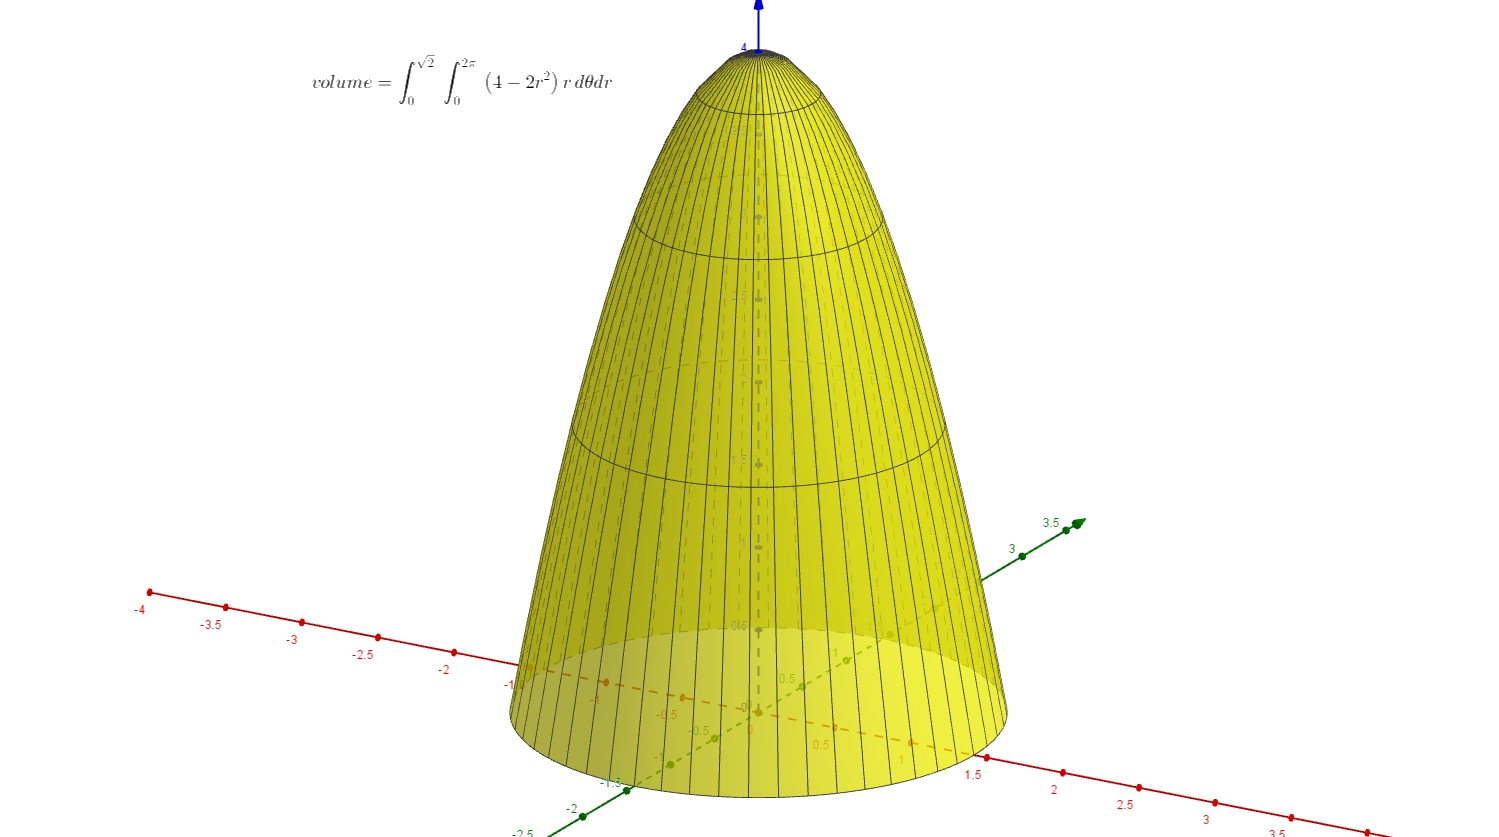
\includegraphics[width=0.5\textwidth]{v13_a03_e01.png}		
	\end{figure}
	
	\begin{align*}
		4 - 2x^2 - 2y^2 = 0 \Rightarrow -2x^2 - 2y^2 = - 4 \Rightarrow - 2\left(x^2 + y^2\right) = -4 \Rightarrow\\ x^2 + y^2 = \dfrac{-4}{-2} = 2 \Rightarrow r = \sqrt{2}
	\end{align*}
	\begin{equation*}
		R = \left\{(r, \theta) \in \mathbb{R}^2 \,|\, 0 \leq r \leq \sqrt{2},\, 0 \leq \theta \leq 2\pi\right\}
	\end{equation*}
	\begin{equation*}
		z = 4 - 2x^2 - 2y^2 = 4 - 2\left(x^2 + y^2\right) = 4 - 2r^2
	\end{equation*}
	\begin{equation*}
		da = dxdy = r\, drd\theta
	\end{equation*}
	\begin{align*}
		\iint_R z\, da = \iint_R \left(4 - 2x^2 - 2y^2\right)\, dxdy = \int_0^{\sqrt{2}} \int_0^{2\pi} \left(4 - 2r^2\right) r\, drd\theta =\\ \int_0^{\sqrt{2}} \left(4r - 2r^3\right) \, dr \int_0^{2\pi} d\theta = \int_0^{\sqrt{2}} \left(4r - 2r^3\right) \, dr [\theta]_0^{2\pi} = 2\pi\int_0^{\sqrt{2}} \left(4r - 2r^3\right) \, dr =\\ 8\pi\int_0^{\sqrt{2}} r\, dr - 4\pi\int_0^{\sqrt{2}} r^3\, dr = \left[\dfrac{8\pi r^2}{2} - \dfrac{\overstrike{4}\pi r^4}{\overstrike{4}}\right]_0^{\sqrt{2}} = \left[4\pi r^2 - \pi r^4\right]_0^{\sqrt{2}} = \left[\pi r^2\left(4 - r^2\right)\right]_0^{\sqrt{2}} =\\ \pi \left(\sqrt{2}\right)^2\left(4 - \left(\sqrt{2}\right)^2\right) = 2\pi(4 - 2) = 4\pi
	\end{align*}
\end{enumerate}